% Chapter Template

\chapter{Ensayos y Resultados} % Main chapter title

\label{Chapter4} % Change X to a consecutive number; for referencing this chapter elsewhere, use \ref{ChapterX}

En este capítulo se describe la estrategia general de \textit{testing} del proyecto y se documentan los ensayos realizados en tres niveles de abstracción: nivel de función, nivel de módulo y nivel de sistema.

%----------------------------------------------------------------------------------------
%	SECTION 1
%----------------------------------------------------------------------------------------

\section{Test Master Plan}
\label{sec:masterPlan}

Para la elaboración de un \textit{Test Master Plan} se tomaron elementos del paradigma de desarrollo basado el pruebas o TDD (por sus siglas en inglés, \textit{Test Driven Development}) como fue mencionado en en capítulo \ref{Chapter2}, subsección \ref{subsec:tdd}. 

Cabe destacar en este sentido, que en la planificación de las tareas del proyecto, primero se definieron los casos de prueba; luego se prepararon las herramientas de \textit{testing}; luego se implementaron los módulos y finalmente, se realizaron las pruebas. Esto puede observarse en el diagrama de \textit{Activity on Node} de la figura \ref{fig:AoN} en la sección \ref{sec:plan}.

Resultó necesario tener bien definidos los requisitos funcionales y sus criterios de aceptación.  Se debieron contemplar todos los casos posibles de uso, tanto exitosos como de error, con lo que se elaboró un documento \citep{TestMasterPlan} de casos de prueba por módulo  y de esta manera, se dio cumplimiento al requerimiento 1.2 indicado en la sección \ref{sec:requerimientos}.  

Se ensayó el código en tres niveles distintos de abstracción: a nivel de función, de módulo y de sistema, según se documenta en las subsecciones \ref{subsec:unitarias} Pruebas unitarias, \ref{subsec:pruebasFuncionales} Pruebas funcionales y \ref{subsec:pruebasSistema} Pruebas de sistema, respectivamente. 

Asimismo, las pruebas sobre los módulos fueron diseñadas para evaluar únicamente la lógica principal de funcionamiento.  En cada caso, se debió abstraer al módulo bajo ensayo de otras capas o servicios que pudieran interactuar con su lógica principal, para lo cual se simuló el resultado de dichas interacciones con \textit{mocks}. 


\subsection{Pruebas unitarias}
\label{subsec:unitarias}

Para realizar pruebas unitarias al código se utilizó el framework Ceedling \citep{ceedling} que se distribuye como una gema del lenguaje de programación ruby.  \textit{Ceedling} integra tres herramientas, \textit{Unity}, \textit{Cmock} y \textit{CException} y se encarga de compilar y ejecutar los \textit{test} sobre el código.

A continuación se presentan los casos de prueba que se definieron para ensayar con \textit{test} unitarios, las funciones de los cuatro módulos desarrollados.  

Se utilizó una técnica para expandir la cantidad de \textit{tests} posibles que consiste en desdoblar el ensayo sobre cada característica a evaluar en al menos tres \textit{tests}: un \textit{test} positivo, un \textit{test} negativo y otro de rango cuando esto último fuera pertinente.  Esto significa evaluar cuando una condición se cumple (positivo) y también cómo reacciona el sistema cuando no se cumple (negativo).  Los \textit{test} de rango permiten evaluar si los parámetros y resultados que devuelven las funciones ensayadas se encuentran dentro de los valores previsto y si se detecta cuando no lo están.

\subsubsection{Módulo Almacenamiento}

En la figura \ref{fig:test_almacenamiento} se recopilan los casos de prueba para el módulo de almacenamiento.  En la primer columna se incluye un código de identificación único del \textit{test} que permite realizar la trazabilidad con los requerimientos.

\begin{figure}[htpb]
	\centering
	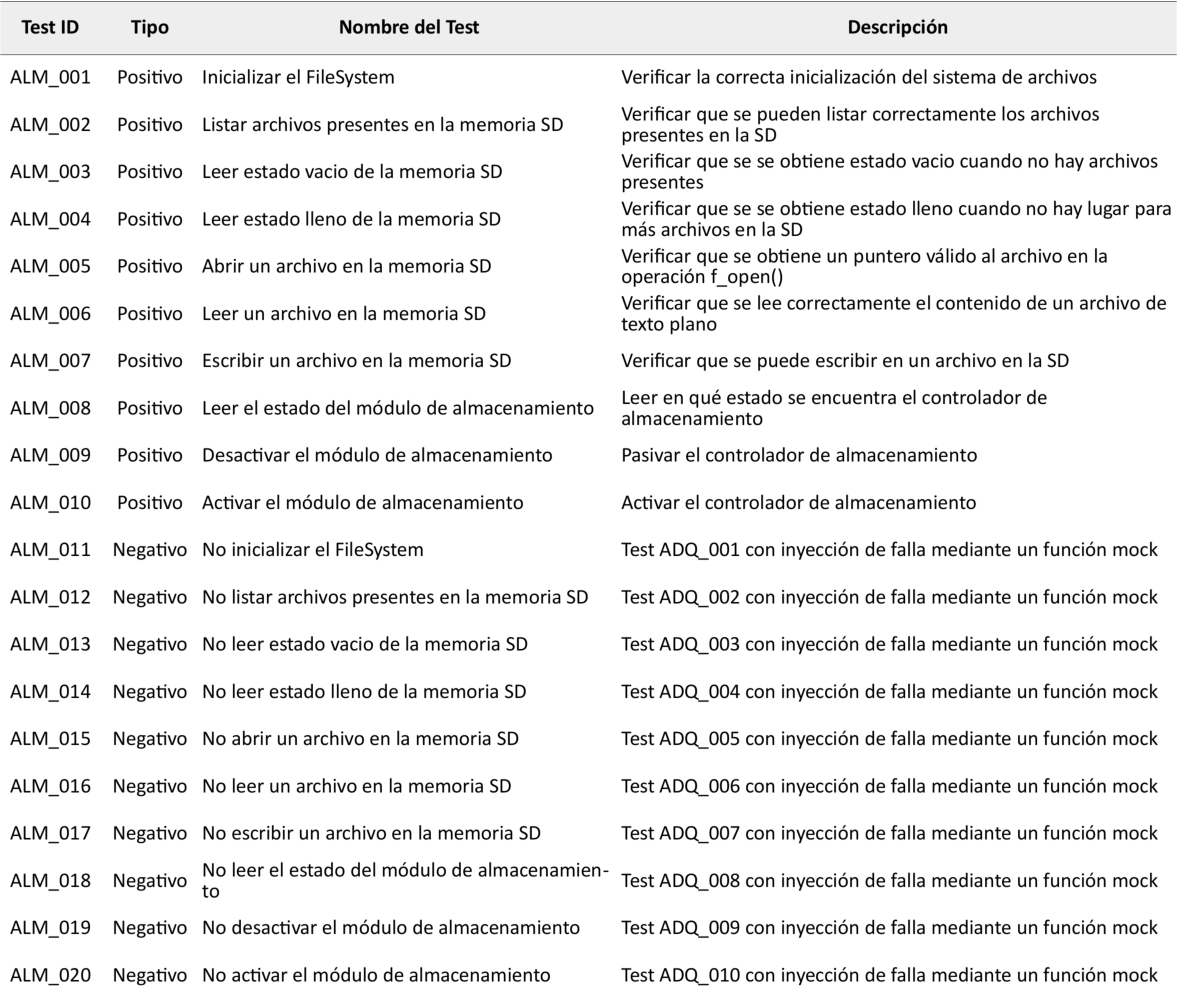
\includegraphics[width=\textwidth]{./Figures/TestSD.pdf}
	\caption{Casos de prueba para \textit{test} unitarios del módulo de almacenamiento}
	\label{fig:test_almacenamiento}
\end{figure}

Los \textit{test} negativos se resolvieron con funciones \textit{mock} que simulan el comportamientos erróneo del componente bajo prueba.  No se realizaron \textit{test} de rango para este módulo.

Todos los \textit{test} ejecutados resultaron exitosos.

\subsubsection{Módulo adquisición}

Los casos de prueba para el módulo de adquisición se presentan en la figura \ref{fig:test_adquisición}. Para este módulo se definieron diez \textit{test} de rango además de los \textit{test} positivos y negativos.  Para éstos últimos se utilizaron funciones \textit{mock} para simular una falla.

\begin{figure}[!htpb]
	\centering
	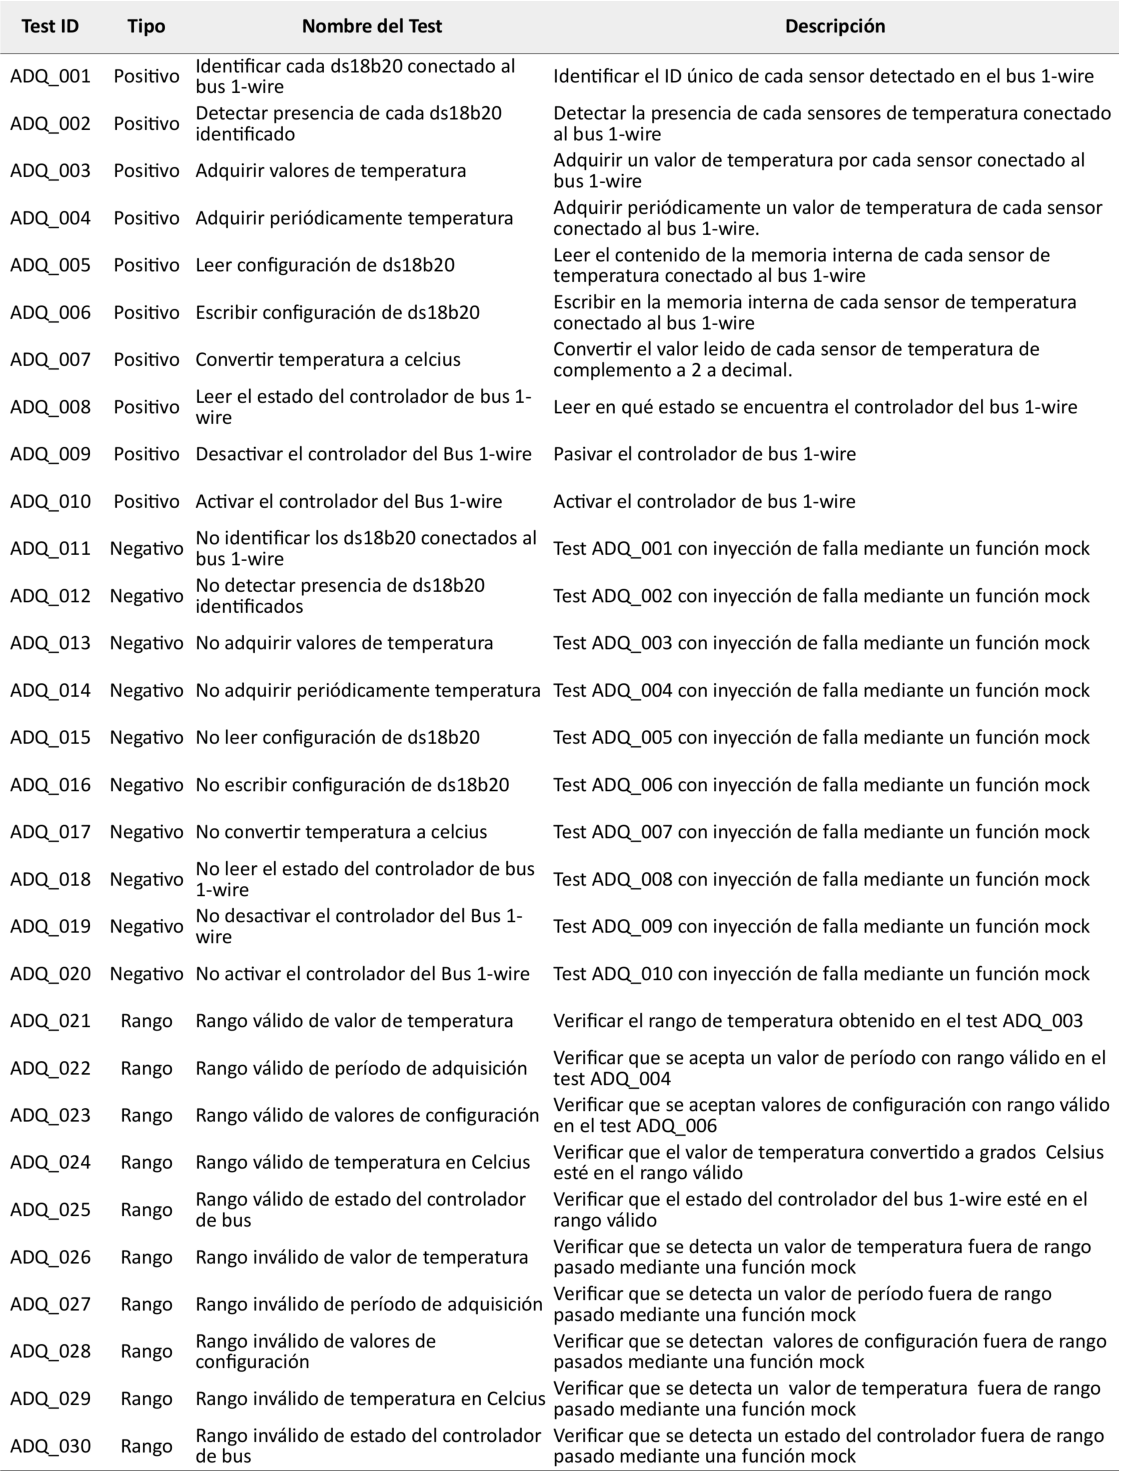
\includegraphics[width=\textwidth]{./Figures/TestADQ.pdf}
	\caption{Casos de prueba para \textit{test} unitarios del módulo de adquisición}
	\label{fig:test_adquisición}
\end{figure}

Todos los \textit{test} ejecutados resultaron exitosos.

\subsubsection{Módulo HMI}


En la figura \ref{fig:test_interfaz} se recopilan los casos de prueba para el módulo de interfaz máquina-hombre.  En la primer columna se incluye un código de identificación único del \textit{test} que permite realizar la trazabilidad con los requerimientos. Los \textit{test} de tipo negativo se implementaron con funciones \textit{mock} para inyectar una falla.

\begin{figure}[htpb]
	\centering
	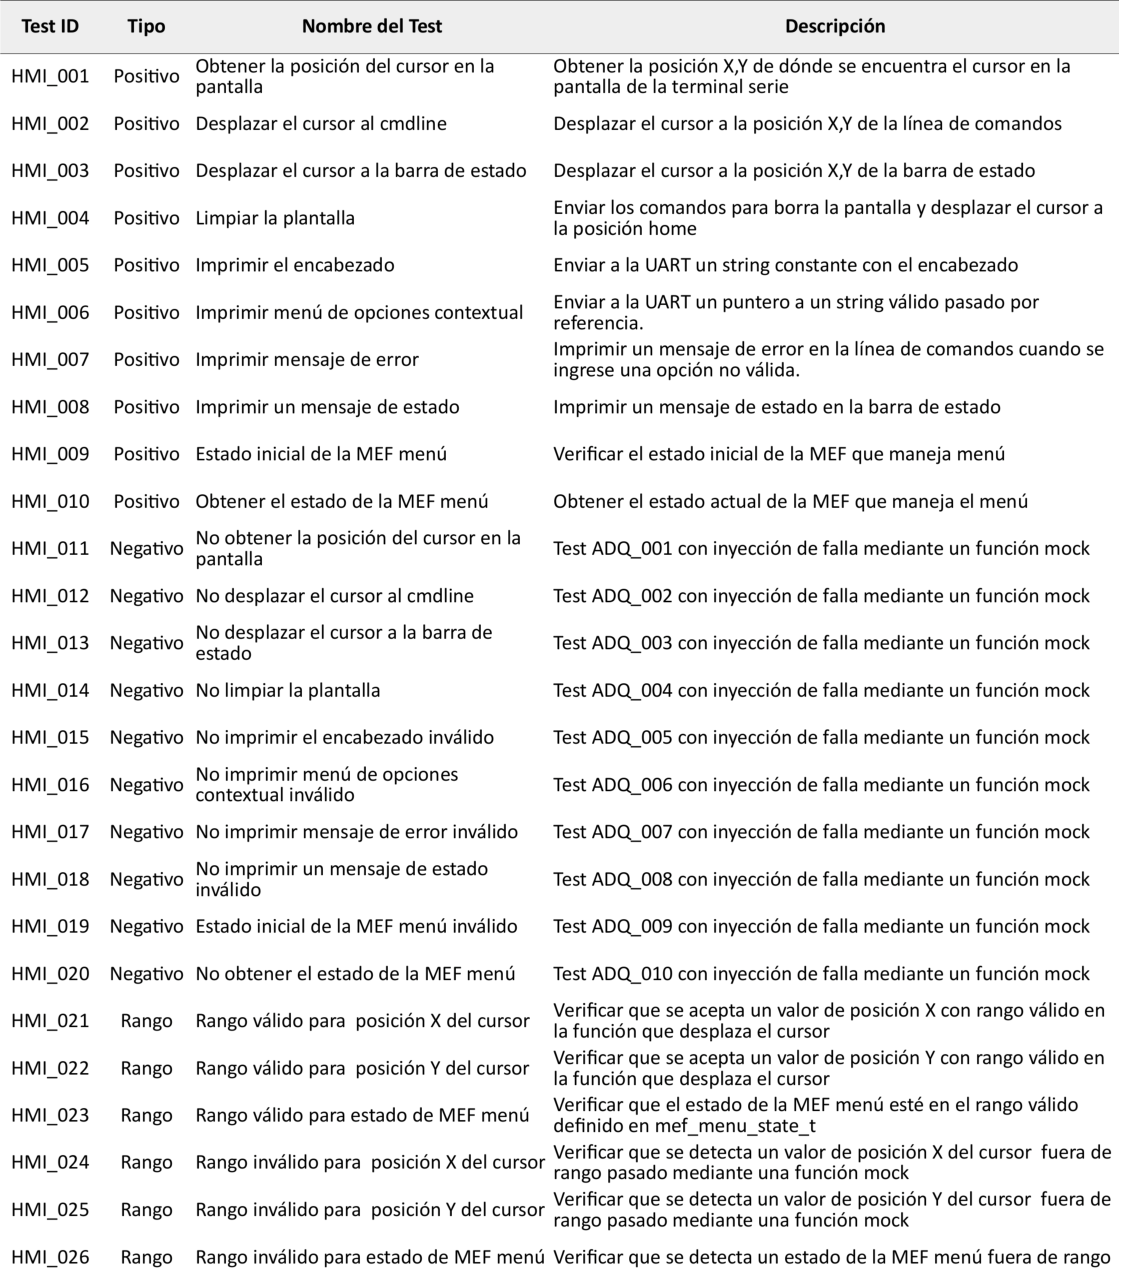
\includegraphics[width=\textwidth]{./Figures/TestHMI.pdf}
	\caption{Casos de prueba para \textit{test} unitarios del módulo de interfaz máquina-hombre}
	\label{fig:test_interfaz}
\end{figure}

Para este módulo se definieron tres \textit{test} de rango válido y tres \textit{test} de rango inválido. Éstos verifican los valores de posición X e Y en la función que desplaza el cursor por la pantalla y el valor de la variable de estado de la MEF que controla el menú de opciones contextual, respectivamente.

Todos los \textit{test} ejecutados resultaron exitosos.

\subsubsection{Módulo Control}

En la figura \ref{fig:test_control} se recopilan los casos de prueba para el módulo de control.  En la primer columna se incluye un código de identificación único del \textit{test} que permite realizar la trazabilidad con los requerimientos. %Los test de tipo negativo se implementaron con funciones \textit{mock} para inyectar una falla.

\begin{figure}[!htpb]
	\centering
	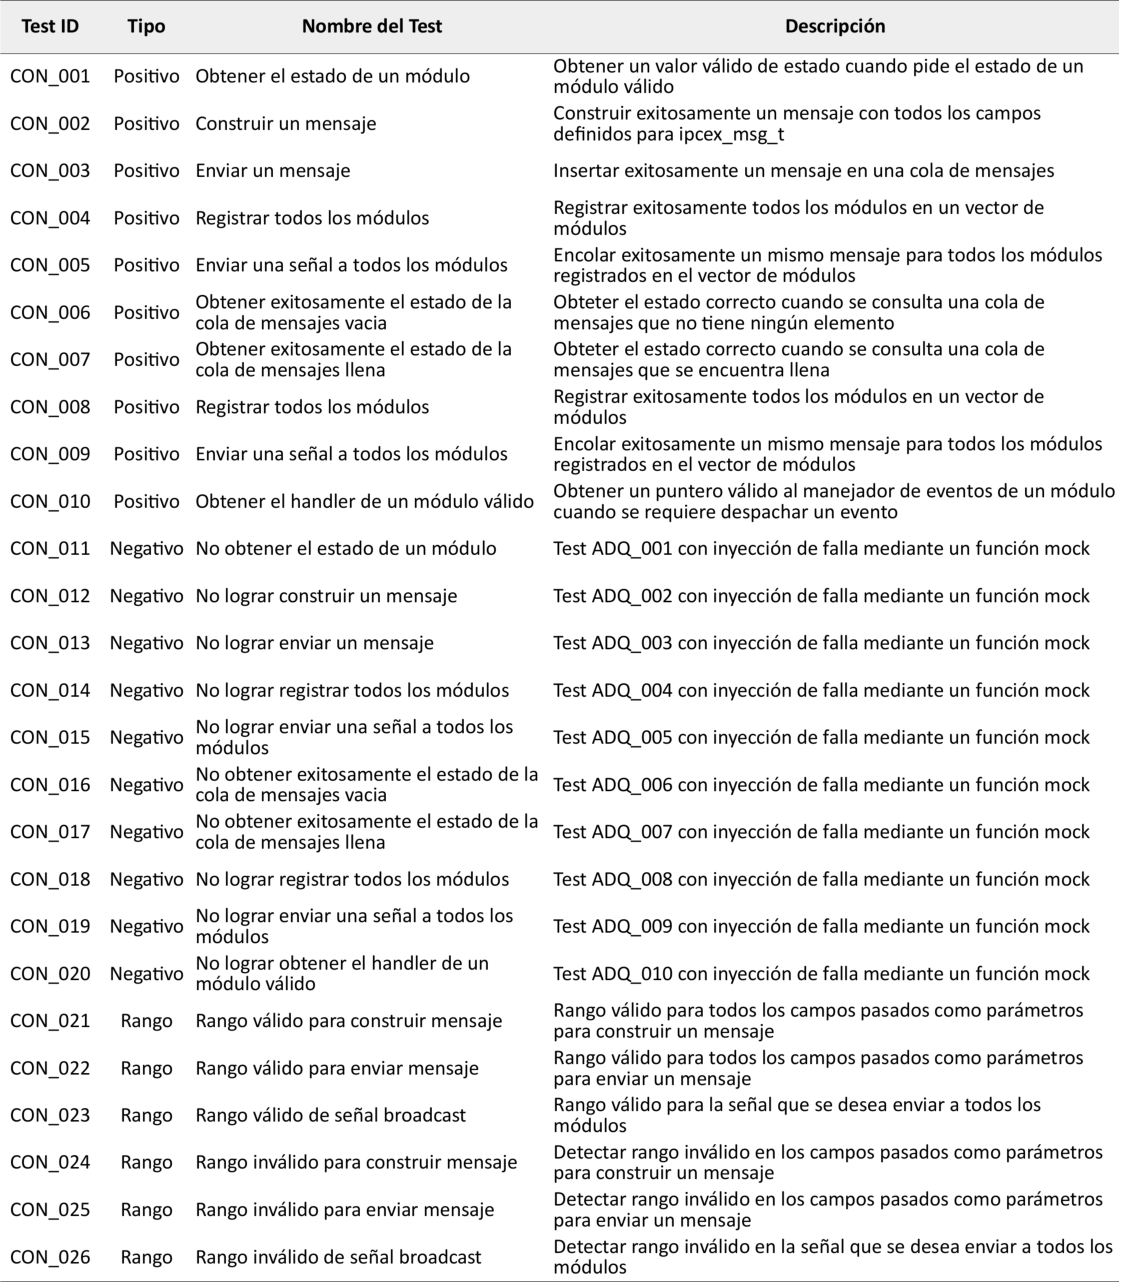
\includegraphics[width=\textwidth]{./Figures/TestCON.pdf}
	\caption{Casos de prueba para \textit{test} unitarios del módulo de control}
	\label{fig:test_control}
\end{figure}

Para este módulo se definieron tres \textit{test} de rango válido y tres \textit{test} de rango inválido. Éstos verifican los valores pasados como parámetros a las funciones para construir y enviar mensajes, y el valor de la señal que se desea enviar a todos los módulos, respectivamente.

Todos los \textit{test} ejecutados resultaron exitosos.

\subsection{Pruebas funcionales}
\label{subsec:pruebasFuncionales}

Se utilizaron pruebas funcionales para el módulo de almacenamiento desarrolladas por Santiago Germino para la sAPI \citep{pruebasfuncionales}.  En particular, se incluyeron en el código del proyecto las funciones \texttt{fatFsFunctionalTest} y \texttt{fatFsTest}. Se realizaron pequeñas modificaciones para adaptar su contenido a la CIAA-NXP, ya que las mismas fueron desarrolladas para ser ejecutadas en la EDU-CIAA-NXP.

La salida de las pruebas se produce por la terminal serie con el resultado que se aprecia en la figura \ref{fig:test_funcional}.

\begin{figure}[htpb]
\begin{center}
\begin{verbatim}

------------------------------------------------
Bienvenido a la prueba de wrappers sdcard/usbms!
------------------------------------------------
Iniciando sdcard con configuracion:
  velocidad inicial 100000 Hz.
  velocidad de trabajo 25000000 Hz.
FSSDC: [InitSPI] New card status: Inserted.
FSSDC: [Init] Initialization begins.
FSSDC: [Init] New card status: Native Mode.
FSSDC: [Init] New card status: Initializing.
FSSDC: [Init] New card status: Ready (Fast Clock).
Inicio de sdcard OK! Unidad FatFs 'SDC:'.
NO se probara usbms.
Logueando STATUS de dipositivos...
STATUS: Tarjeta SD lista y montada.

-------------------------------------------
TEST sobre archivo 'SDC:/TEST.TXT'.
-------------------------------------------
TEST: Ejecutando 'f_open( WRITE )'...OK!
TEST: Ejecutando 'f_putc'...OK!
TEST: Ejecutando 'f_puts'...OK!
TEST: Ejecutando 'f_open( READ )'...OK!
TEST: Ejecutando 'f_read'...OK!

>>>> INICIO CONTENIDO DEL ARCHIVO LEIDO >>>>
La unidad bajo prueba es 'SDC:'
Lista de caracteres ASCII:
 !"#$%&'()*+,-./0123456789:;<=>?@ABCDEFGHIJKLMNOPQRSTUVWXYZ
 [\]^_`abcdefghijklmnopqrstuvwxyz{|}~
Fecha y hora de compilacion: Nov 22 2018 18:59:47
Estado de Salidas Digitales DO0 a DO3 en la prueba: 1111
<<<< FIN CONTENIDO DEL ARCHIVO LEIDO <<<<
--------
TEST OK!
--------
**FIN**
\end{verbatim}
\end{center}
\caption{Salida por consola del test funcional para el módulo de almacenamiento}
\label{fig:test_funcional}
\end{figure}


%Se incluyeron en el código del proyecto las funciones que implementan los tests funcionales con los siguientes prototipos:
%
%\begin{itemize}
%	\item \texttt{void fatFsFunctionalTest( void );}
%	\item \texttt{static bool fatFsTest( const char *unidad );}
%\end{itemize} 


En el algoritmo \ref{lst:funcional} se incluye la versión adaptada de la función original que implementa los \textit{test} funcionales y cuya salida fue mostrada en la figura \ref{fig:test_funcional}. %en los cuales se utilizan los diferentes modos de lectura y escritura sobre la tarjeta microSD.

\begin{lstlisting}[caption={Código para las puebas funcionales para el módulo de almacenamiento.},label={lst:funcional}]
static bool fatFsTest( const char *unidad )
{
	char buf[1024];
	char filename[64];
	FIL file;
	FRESULT fr;
	int r;

	sprintf( filename, "%s/TEST.TXT", unidad );

	uartWriteString( UART_USB, "\r\n-------------------------------------------\r\n" );
	sprintf( buf, "TEST sobre archivo '%s'.\r\n", filename);
	uartWriteString( UART_USB, buf);
	uartWriteString( UART_USB, "-------------------------------------------\r\n" );

	// Ver http://elm-chan.org/fsw/ff/00index_e.html 
	// para una referencia de la API de FatFs

	// Abre un archivo. Si no existe lo crea, si existe, lo sobreescribe.
	fatFsTestStart( "f_open( WRITE )" );
	fr = f_open( &file, filename, FA_CREATE_ALWAYS | FA_WRITE);
	if( fr != FR_OK )
	{
		fatFsTestERROR( fr );
		return false;
	}
	fatFsTestOK( );

	// Prueba de f_putc
	fatFsTestStart( "f_putc" );
	sprintf (buf, "La unidad bajo prueba es '%s'\r\n"
			"Lista de caracteres ASCII:\r\n", 	unidad);
	// Escribe mensaje
	for (uint32_t i = 0; i < strlen(buf); ++i) {
		r = f_putc( buf[i], &file );
		if (r < 1)
		{
			fatFsTestERROR( r );
			f_close( &file );
			return false;
		}
	}

	// Escribe todos los caracteres UTF-8 que overlapean ASCII
	// (sin combinaciones multibyte)
	for (uint32_t i = 32; i < 127; ++i)
	{
		r = f_putc( (TCHAR)i, &file );
		if (r < 1)
		{
			fatFsTestERROR( r );
			f_close( &file );
			return false;
		}
	}
	fatFsTestOK( );

	// Prueba f_puts
	fatFsTestStart( "f_puts");
	sprintf (buf, "\r\n"
			"Fecha y hora de compilacion del programa: %s %s\r\n"
			"Estado de Salidas Digitales DO0 a DO3 en la prueba: %i%i%i%i\r\n",
			__DATE__, __TIME__,
			gpioRead( DO0 ), gpioRead( DO1 ), gpioRead( DO2 ), gpioRead( DO3 ));

	r = f_puts( buf, &file );
	if (r < 1)
	{
		fatFsTestERROR( r );
		f_close( &file );
		return false;
	}
	fatFsTestOK( );

	// Cierra el archivo y vuelve a abrirlo como LECTURA
	f_close( &file );

	fatFsTestStart( "f_open( READ )" );
	fr = f_open( &file, filename, FA_READ );
	if( fr != FR_OK )
	{
		fatFsTestERROR( fr );
		return false;
	}
	
	fatFsTestOK( );

	// Borro contenido del buffer, para que no haya 
	// dudas de que el contenido se leyo desde el archivo
	memset( buf, 0, sizeof(buf) );

	// Carga el contenido del archivo
	UINT bytesLeidos = 0;
	fatFsTestStart( "f_read" );
	fr = f_read( &file, buf, sizeof(buf), &bytesLeidos );
	if (fr != FR_OK)
	{
		fatFsTestERROR( fr );
		return false;
	}
	fatFsTestOK( );

	f_close( &file );

	uartWriteString( UART_USB, "\r\n");
	uartWriteString( UART_USB, ">>>> INICIO CONTENIDO DEL ARCHIVO LEIDO >>>>\r\n");
	uartWriteString( UART_USB, buf );
	uartWriteString( UART_USB, "<<<< FIN CONTENIDO DEL ARCHIVO LEIDO <<<<\r\n");
	return true;
}
\end{lstlisting}


\subsection{Pruebas de sistema}
\label{subsec:pruebasSistema}

Las pruebas que se presentan en esta sección son las de mayor nivel de abstracción, es decir que evaluan el funcionamiento del código a nivel de sistema con todos los módulos ya integrados al \textit{firmware} y en pleno funcionamiento.

Se permiten las interacciones reales entre los módulos y entre éstos y las distintas capas y servicios que componen el código.  En otras palabras, no se utiliza ningún \textit{mock} para estos ensayos.

Se utilizó el modelo de casos de uso para plantear escenarios representativos del funcionamiento esperado del sistema, de modo que pueda ser evaluado su correcto desenvolvimiento.  Se procuró que estos escenarios estuvieran fuertemente vinculados con los requerimientos funcionales planteados en la sección \ref{sec:requerimientos}.

Al final de esta sección se incluye una matriz de trazabilidad entre los requerimientos funcionales y las pruebas de integración que se detallan en la presente sección.  

Para la construcción de las pruebas a nivel de sistema se confeccionó una plantilla que se adjunta a la memoria en el apendice \ref{AppendixA}.

El primer caso de prueba, identificado con ID UC01, evalua el escenario principal de funcionamiento con la configuración por defecto con que inicia el sistema al ser energizado. Esto es, todos los módulos habilitados y adquisición de temperatura en forma periódica cada 1000 ms.  En la figura \ref{fig:useCase1} se puede apreciar la planilla utilizada para el ensayo. 

\begin{figure}[!htb]
	\centering
	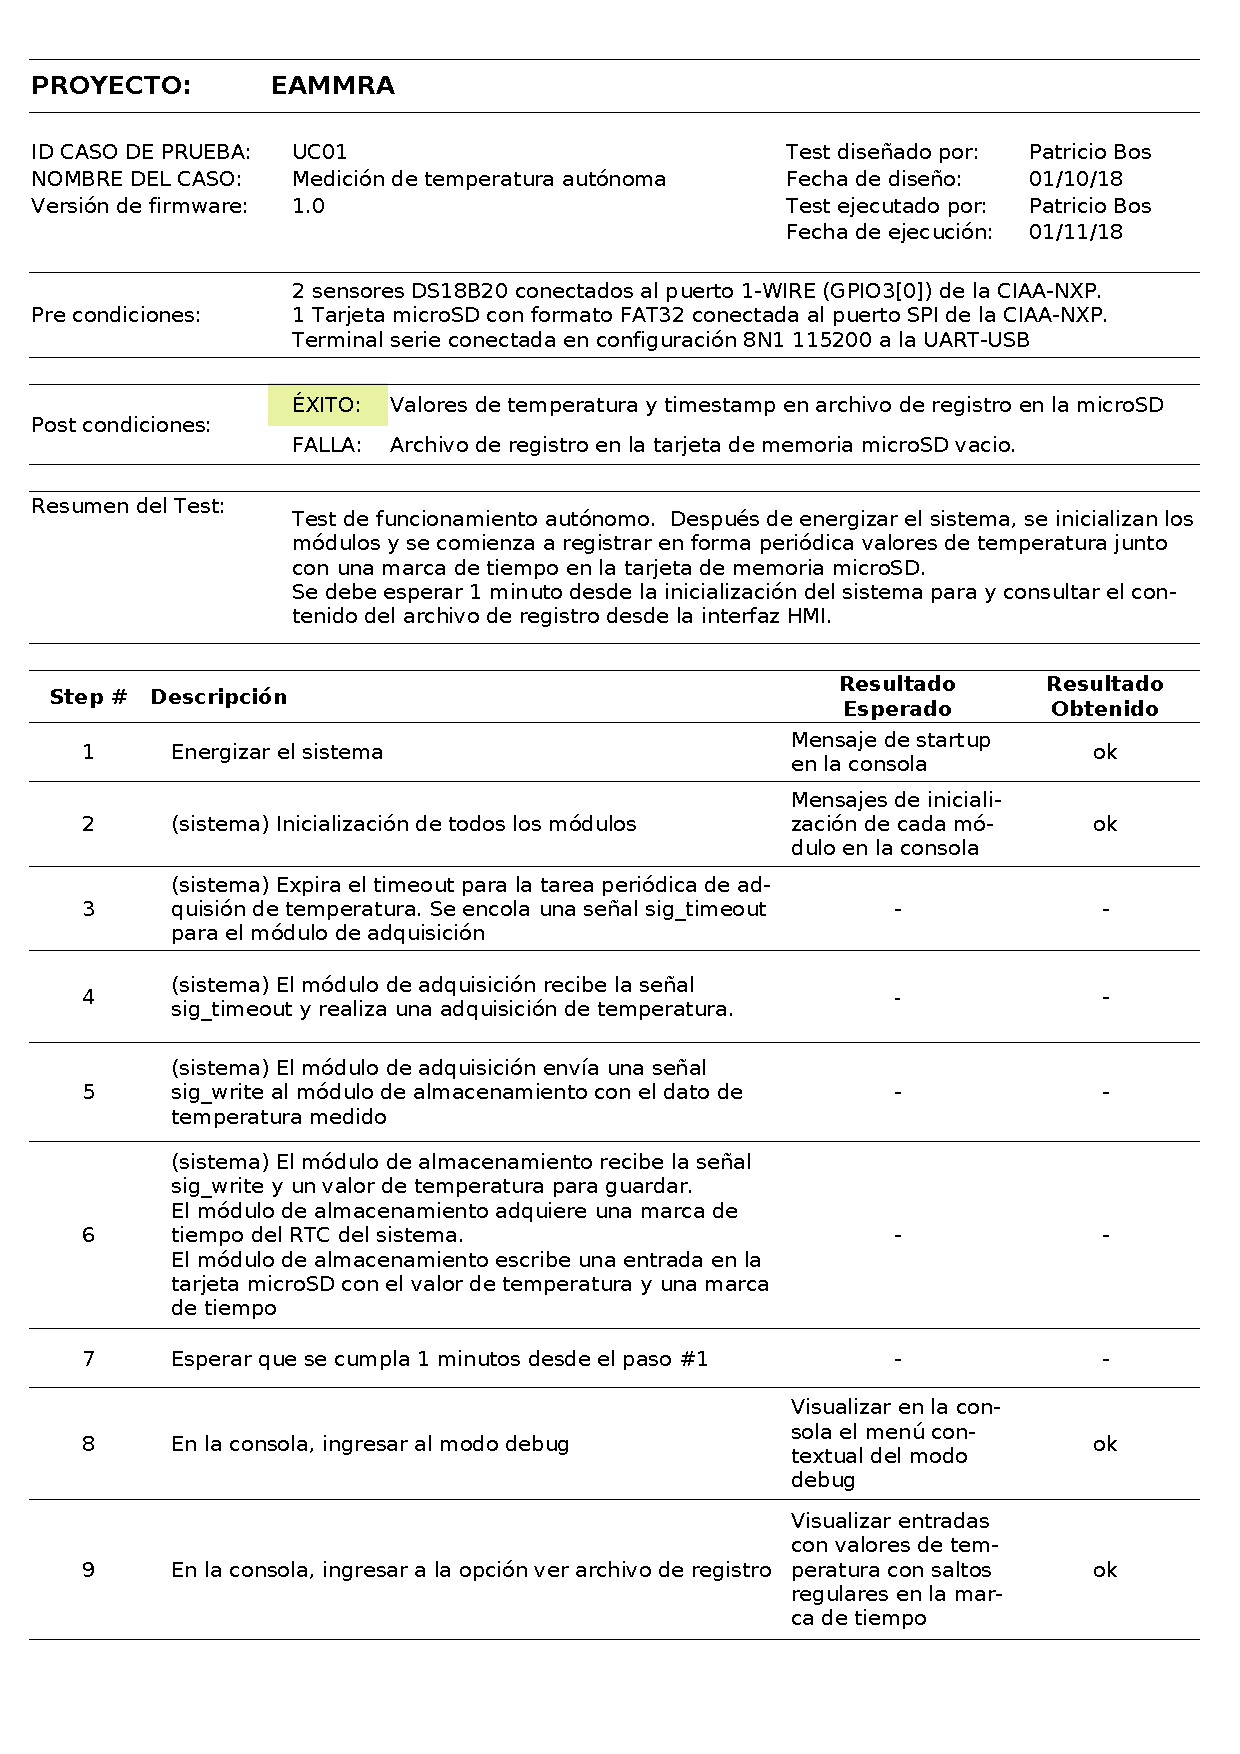
\includegraphics[width=1\textwidth]{./Figures/UseCase1.pdf}
%	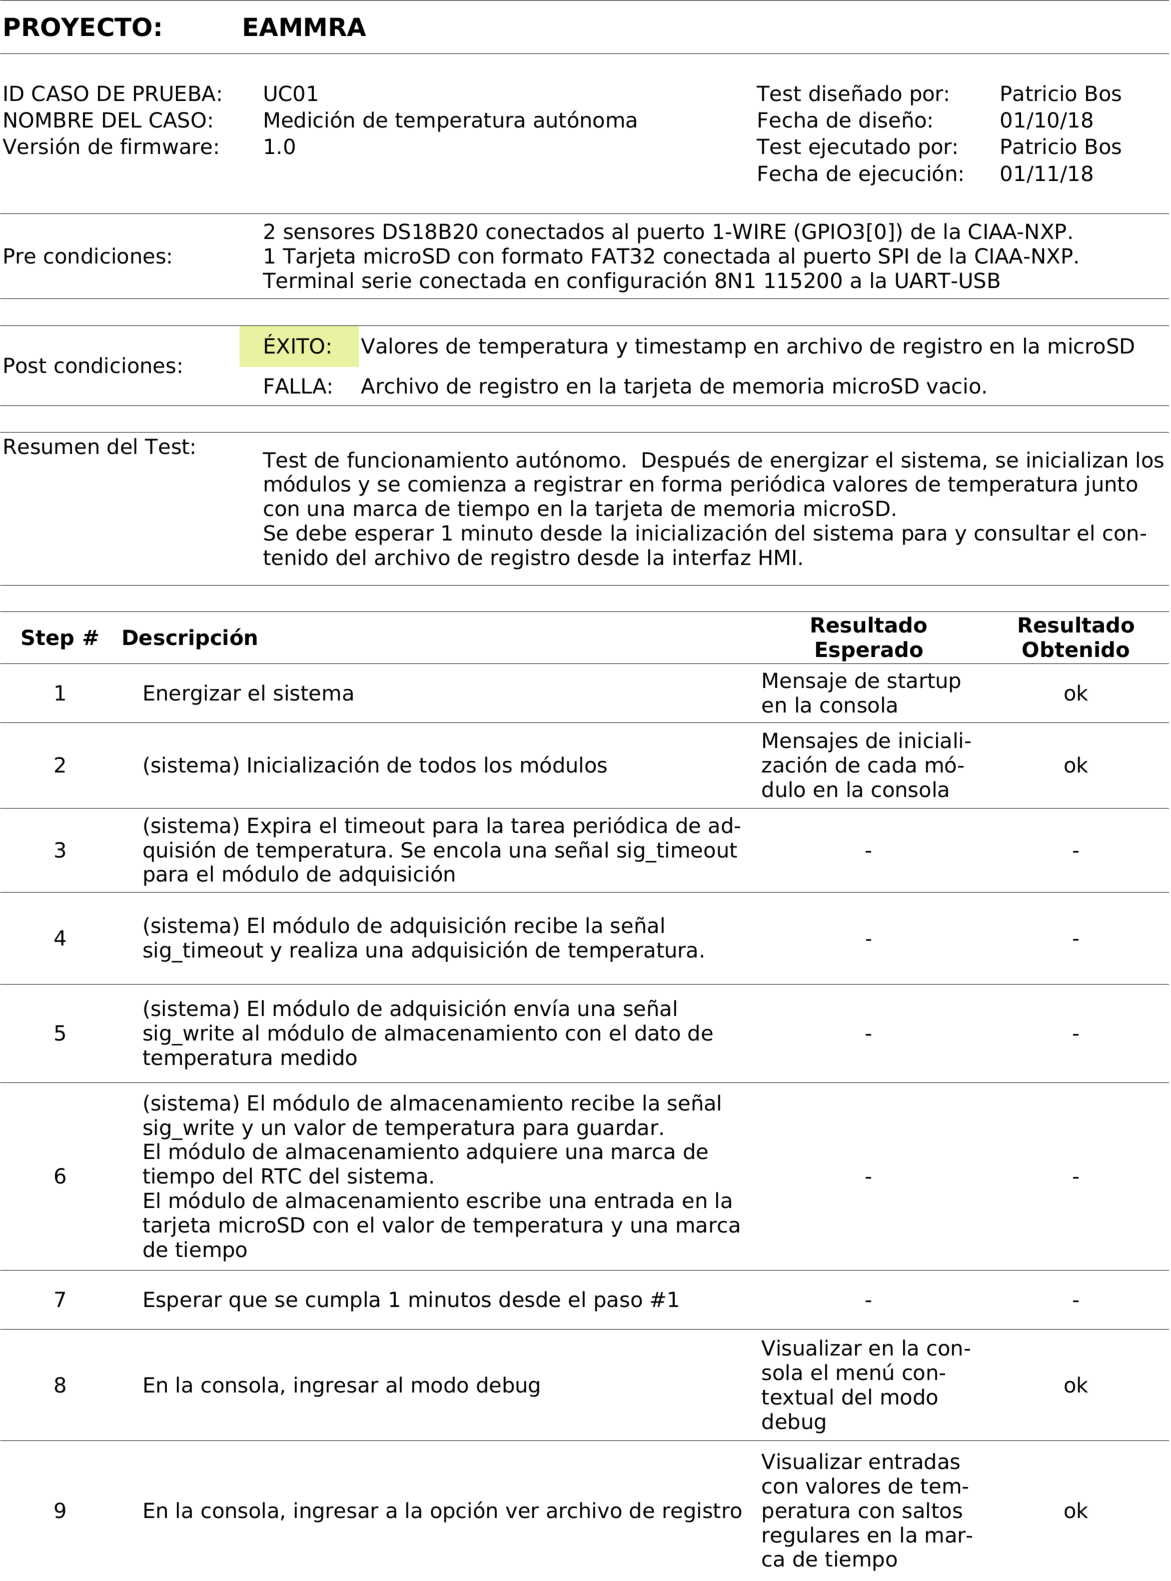
\includegraphics[width=1\textwidth]{./Figures/UseCase1_recortada.pdf}
	\caption{Planilla de caso de uso UC01. Medición autónoma de temperatura en forma periódica. Se indica en color verde la post condición de éxito del ensayo.}
	\label{fig:useCase1}
\end{figure}

Se pudieron validar todos los pasos y el ensayo resultó exitoso.

El segundo caso de prueba, identificado con ID UC02 evalua un escenario en donde el usuario interactua con el sistema para modificar el período de adquisición de valores de temperatura.  Los detalles del ensayo y los resultados obtenidos se presentan en la planilla que se utilizó para la prueba, que se muestra en la figura \ref{fig:useCase2}. 

\vspace{10px}

\begin{figure}[!htb]
	\centering
	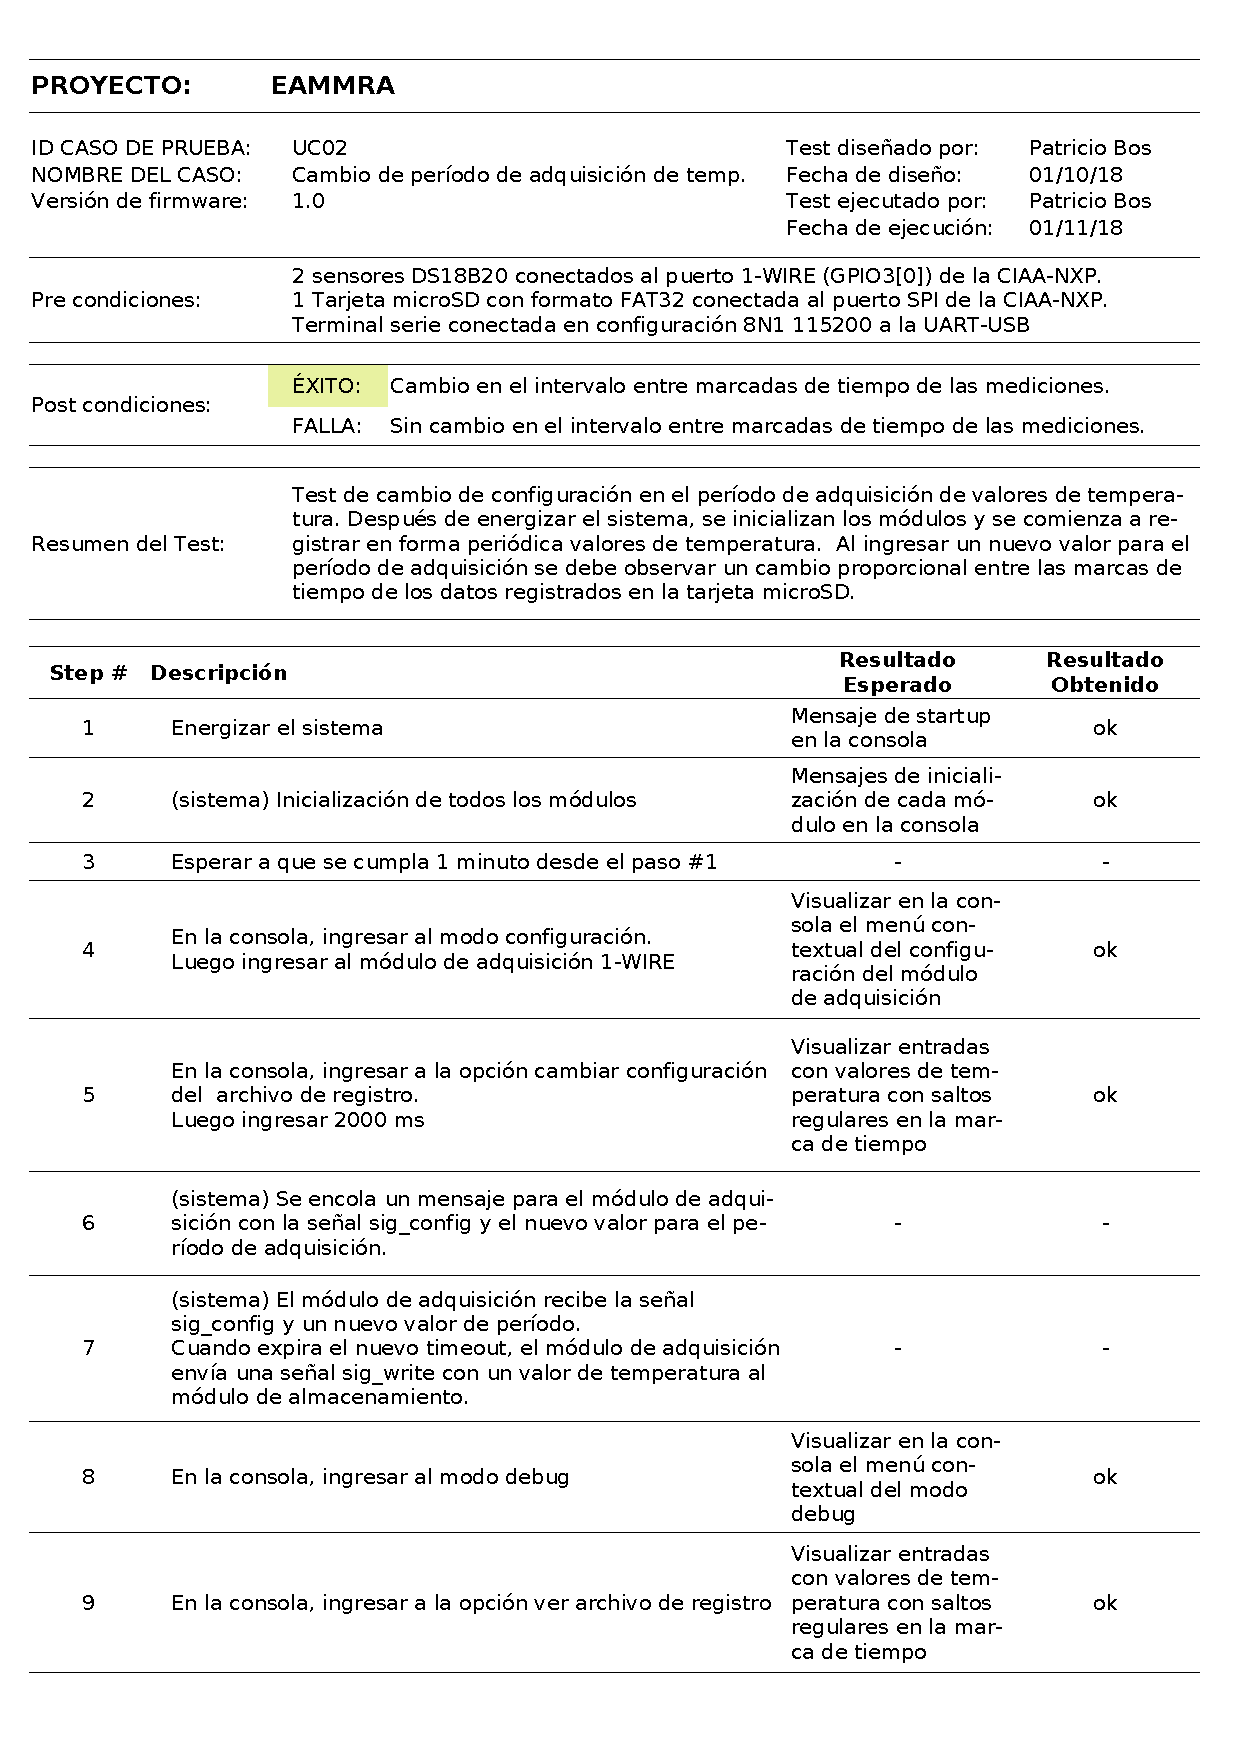
\includegraphics[width=1\textwidth]{./Figures/UseCase2.pdf}
	\caption{Planilla de casos de uso UC02.  Cambio de período de adquisición de valores de temperatura. Se indica en color verde la post condición de éxito del ensayo.}
	\label{fig:useCase2}
\end{figure}

Se pudieron validar todos los pasos y el ensayo resultó exitos.

En la figura \ref{fig:useCase2} se presenta los detalles del tercer caso de prueba, identificado con ID UC03.  En este ensayo se evalua un escenario en donde el usuario interactua con el sistema para modificar el perfil de consumo de energía de la estación. 

En caso de éxito, se observa un último mensaje a través de la interfaz que confirma el cambio de configuración y ésta deja de estar operativa.

\vspace{10px}

\begin{figure}[!htb]
	\centering
	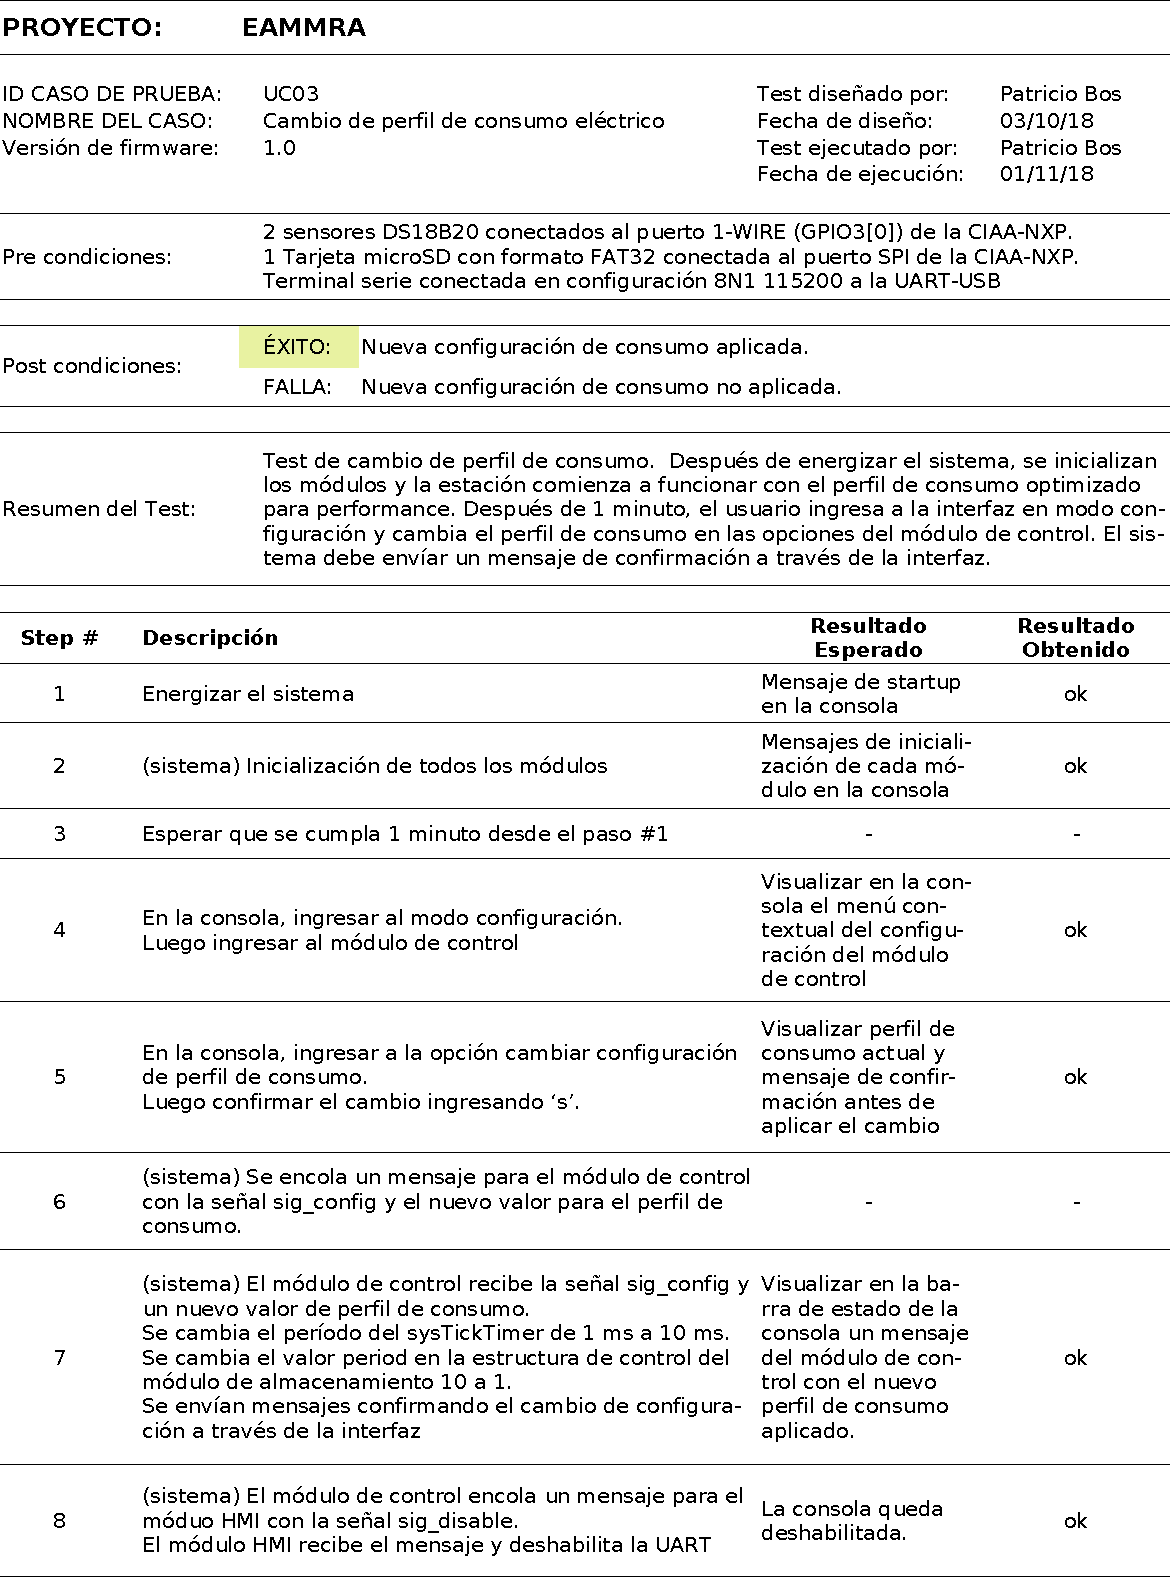
\includegraphics[width=1\textwidth]{./Figures/UseCase3.pdf}
	\caption{Planilla de casos de uso UC03.  Cambio de perfil de consumo de energía. Se indica en color verde la post condición de éxito del ensayo.}
	\label{fig:useCase3}
\end{figure}

Se pudieron validar todos los pasos y el ensayo resultó exitoso.

Se elaboró una matriz de trazabilidad de requerimientos con las pruebas de sistema para controlar fehacientemente que se pudieron alcanzar los requerimientos funcionales como se observa en la tabla \ref{tab:trazabilidad_test}. 

\begin{table}[ht]
\centering
\caption{Matriz de trazabilidad de requerimientos con test de casos de uso.}
\label{tab:trazabilidad_test}
\begin{tabular}{lccc}
\toprule
\textbf{Requerimiento}					   & \textbf{UC01} 	  & \textbf{UC02}  & \textbf{UC03}  \\ \midrule
2.1 Adquirir temperatura                   & X                & X              &    		 	\\ %\hline
2.2 Adquirir velocidad de viento           &                  &                &   		  		\\ %\hline
2.3 Almacenar datos                        & X                & X              &      			\\ %\hline
2.4 Perfiles de consumo                    &                  &                & X    			\\ %\hline
2.5 Interfaz                               & X                & X              & X    			\\ 
\bottomrule
\end{tabular}
\end{table}

Cabe destacar que el requerimiento 2.2, referido a la adquisición de valores de velocidad de viento, no fue evaluado en ningún caso de uso.  Esto responde a que dicho requerimiento no fue implementado.  Cuando esta característica sea finalmente incluida en el sistema se contempla definir dos nuevos casos de uso que la utilice, uno para evaluar la adquisición periódica y otro para evaluar la posibilidad de cambiar dicho período.

Finalmente, en la tabla \ref{tab:trazabilidad_test} puede apreciarse que todos los requerimientos implementados están evaluados por al menos dos casos de uso.  Asimismo, debe notarse que si bien los casos de uso UC01 y UC02 cubren los mismos requerimientos, éstos prueban distintos aspectos del requerimiento 2.1.  UC01 evalua la adquisición periódica de valores de temperatura y UC02 la posibilidad de modificar dicho período de adquisición.